\documentclass[letterpaper, 8pt]{extarticle}
\usepackage{amssymb,amsmath,amsthm,amsfonts}
\usepackage{multicol,multirow}
\usepackage{calc}
\usepackage{ifthen}
\usepackage[landscape]{geometry}
\usepackage[colorlinks=true,citecolor=blue,linkcolor=blue]{hyperref}
\usepackage{booktabs}
\usepackage{ulem}
\usepackage{enumitem}
\usepackage{tabulary}
\usepackage{graphicx}
\usepackage{siunitx}
\usepackage{tikz}
\usepackage{derivative}
\usepackage{svg}
\usepackage{listings}
\usepackage{color}
\usepackage{soul}
\usepackage{clrscode3e}


\ifthenelse{\lengthtest { \paperwidth = 11in}}
    { \geometry{top=.25in,left=.25in,right=.25in,bottom=.3in} }
	{\ifthenelse{ \lengthtest{ \paperwidth = 297mm}}
		{\geometry{top=1cm,left=1cm,right=1cm,bottom=1cm} }
		{\geometry{top=1cm,left=1cm,right=1cm,bottom=1cm} }
	}

\newenvironment{Figure}
  {\par\medskip\noindent\minipage}
  {\endminipage\par\medskip}

\pagestyle{empty}
\makeatletter
\renewcommand{\section}{\@startsection{section}{1}{0mm}%
                                {-1ex plus -.5ex minus -.2ex}%
                                {0.5ex plus .2ex}%x
                                {\normalfont\normalsize\bfseries}}
\renewcommand{\subsection}{\@startsection{subsection}{2}{0mm}%
                                {-1explus -.5ex minus -.2ex}%
                                {0.5ex plus .2ex}%
                                {\normalfont\small\bfseries}}
\renewcommand{\subsubsection}{\@startsection{subsubsection}{3}{0mm}%
                                {-1ex plus -.5ex minus -.2ex}%
                                {1ex plus .2ex}%
                                {\normalfont\tiny\bfseries}}
\makeatother
\setcounter{secnumdepth}{0}
\setlength{\parindent}{0pt}
\setlength{\parskip}{0pt plus 0.5ex}
% -----------------------------------------------------------------------
% \tymin=37pt
% \tymax=\maxdimen

% Custom siunitx defs
\DeclareSIUnit\noop{\relax}

\NewDocumentCommand\prefixvalue{m}{%
\qty[prefix-mode=extract-exponent,print-unity-mantissa=false]{1}{#1\noop}
}

% Shorthand definitions
% \newcommand{\To}{\Rightarrow}

% condense itemize & enumerate
\let\olditemize=\itemize \let\endolditemize=\enditemize \renewenvironment{itemize}{\olditemize \itemsep0em}{\endolditemize}
\let\oldenumerate=\enumerate \let\endoldenumerate=\endenumerate \renewenvironment{enumerate}{\oldenumerate \itemsep0em}{\endoldenumerate}

\title{2GA3}

\begin{document}

\raggedright
\tiny

\begin{center}
	{\textbf{2GA3}} \\
\end{center}
\begin{multicols*}{4}
	\setlength{\premulticols}{1pt}
	\setlength{\postmulticols}{1pt}
	\setlength{\multicolsep}{1pt}
	\setlength{\columnsep}{2pt}

	\section{Logic Basics}
	\subsection{Physics}
	\textbf{Ohm's Law:} $R = \frac{U}{T}$
	\textbf{Series Resistors:} $R = \sum_{i=1}^N R_i$
	\textbf{Parallel Resistors:} $1/R = \sum_{i=1}^N (1/R_i)$
	\subsection{Transistors}
	% REVIEW: Do we want an image here?
	MOSFETs have 4 components: Source, Gate, Drain, and Base

	\textbf{PNP:} Is on when gate is positive. Does not have circle.
	\textbf{NPN:} Is on when gate is negative. Has circle.

	Generally, transistors are used to pull the output to either
	a positive voltage, or a zero voltage (1 or 0, on or off).
	If output is not pulled to one of these,
	the output is floating and is indeterminate in voltage.

	\subsection{Logic Circuits}
	\subsubsection{Symbols}

	% REVIEW: No clue if these are readable, needs to be printed
	% and double checked before release
	\begin{center}
		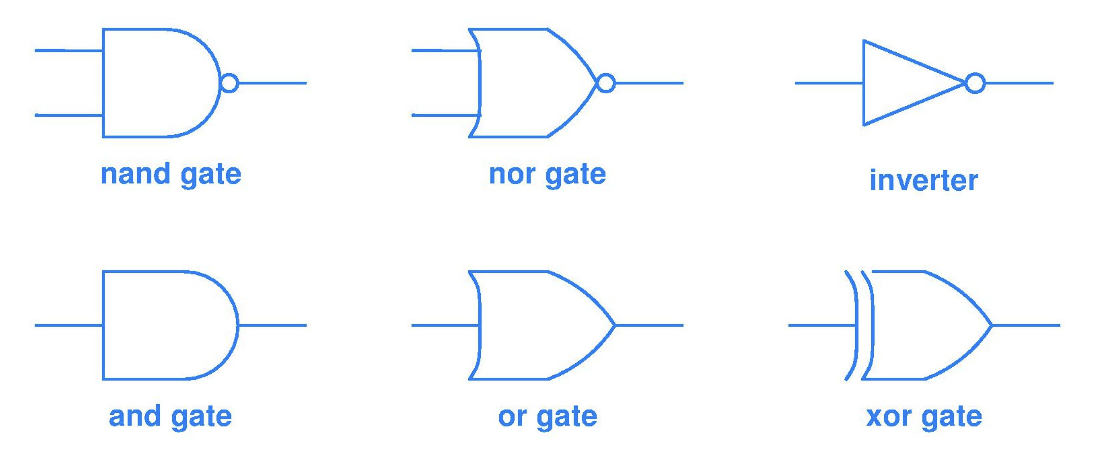
\includegraphics[width=.8\linewidth]{logic-gates.png}
	\end{center}
	\subsubsection{Adders}
	\begin{center}
		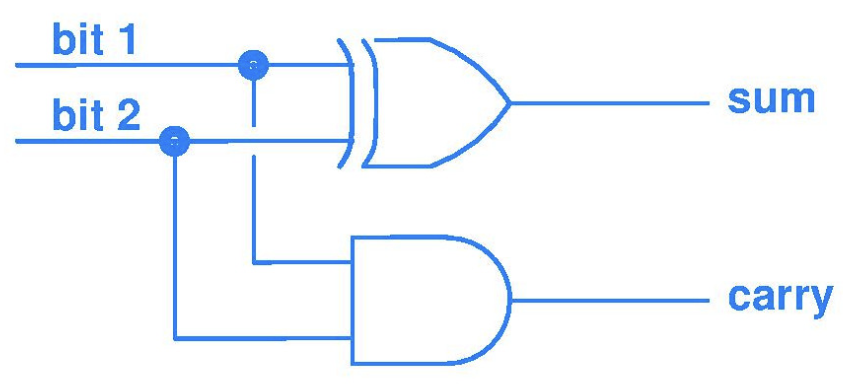
\includegraphics[width=.3\linewidth]{half-adder.png}
		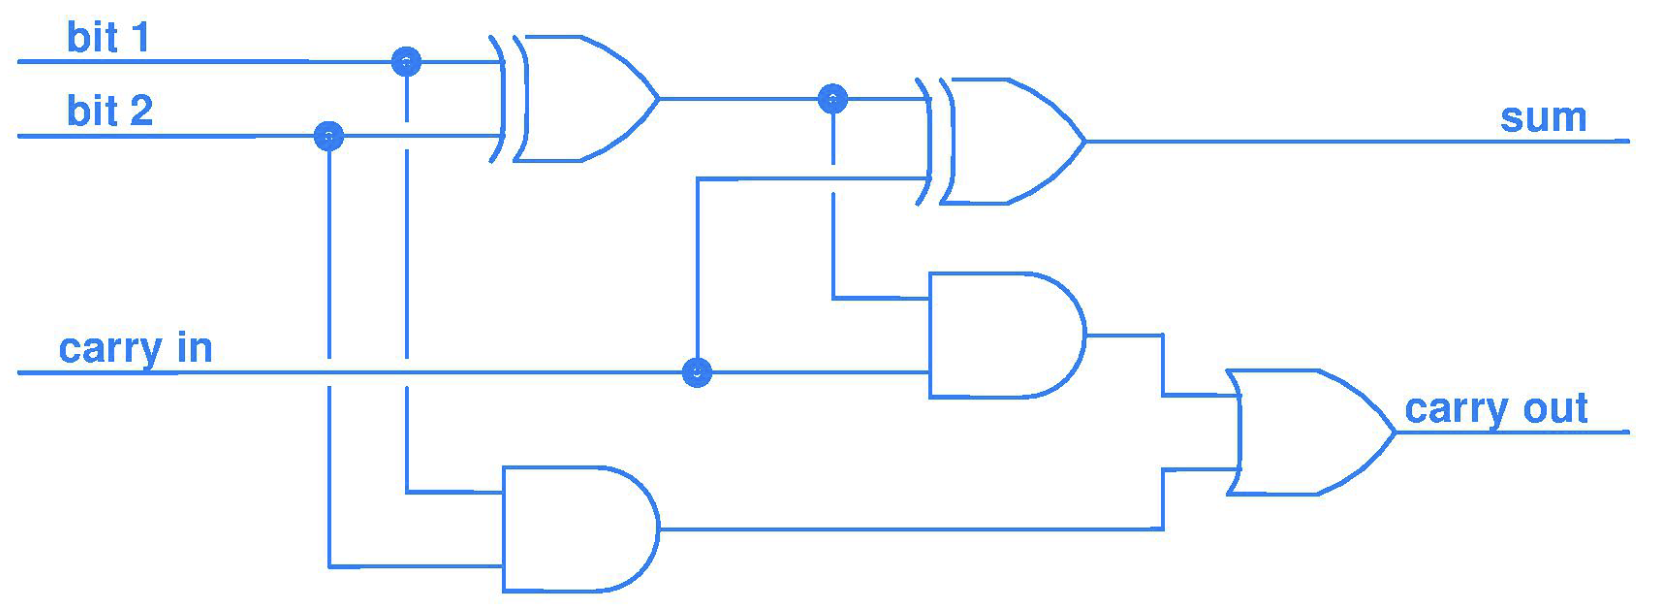
\includegraphics[width=.6\linewidth]{full-adder.png}
		Left: Half-adder. Right: Full-adder.
	\end{center}
	% REVIEW: Is there anything else that needs to be added here?
	Half adders have no way to carry input from previous sums.
	To add more bits, just chain multiple full-adders together using the carry-out
	bit.
	If final carry at end is 1, that signifies an overflow error.

	\subsubsection{Latches \& Flip-flops}
	\textbf{Flip-flop}
	Every time the input switches from 0 to 1, the output switches to the opposite.
	% TODO: Add more detail about flip-flops

	\textbf{Gated D-latch}
	\begin{center}
		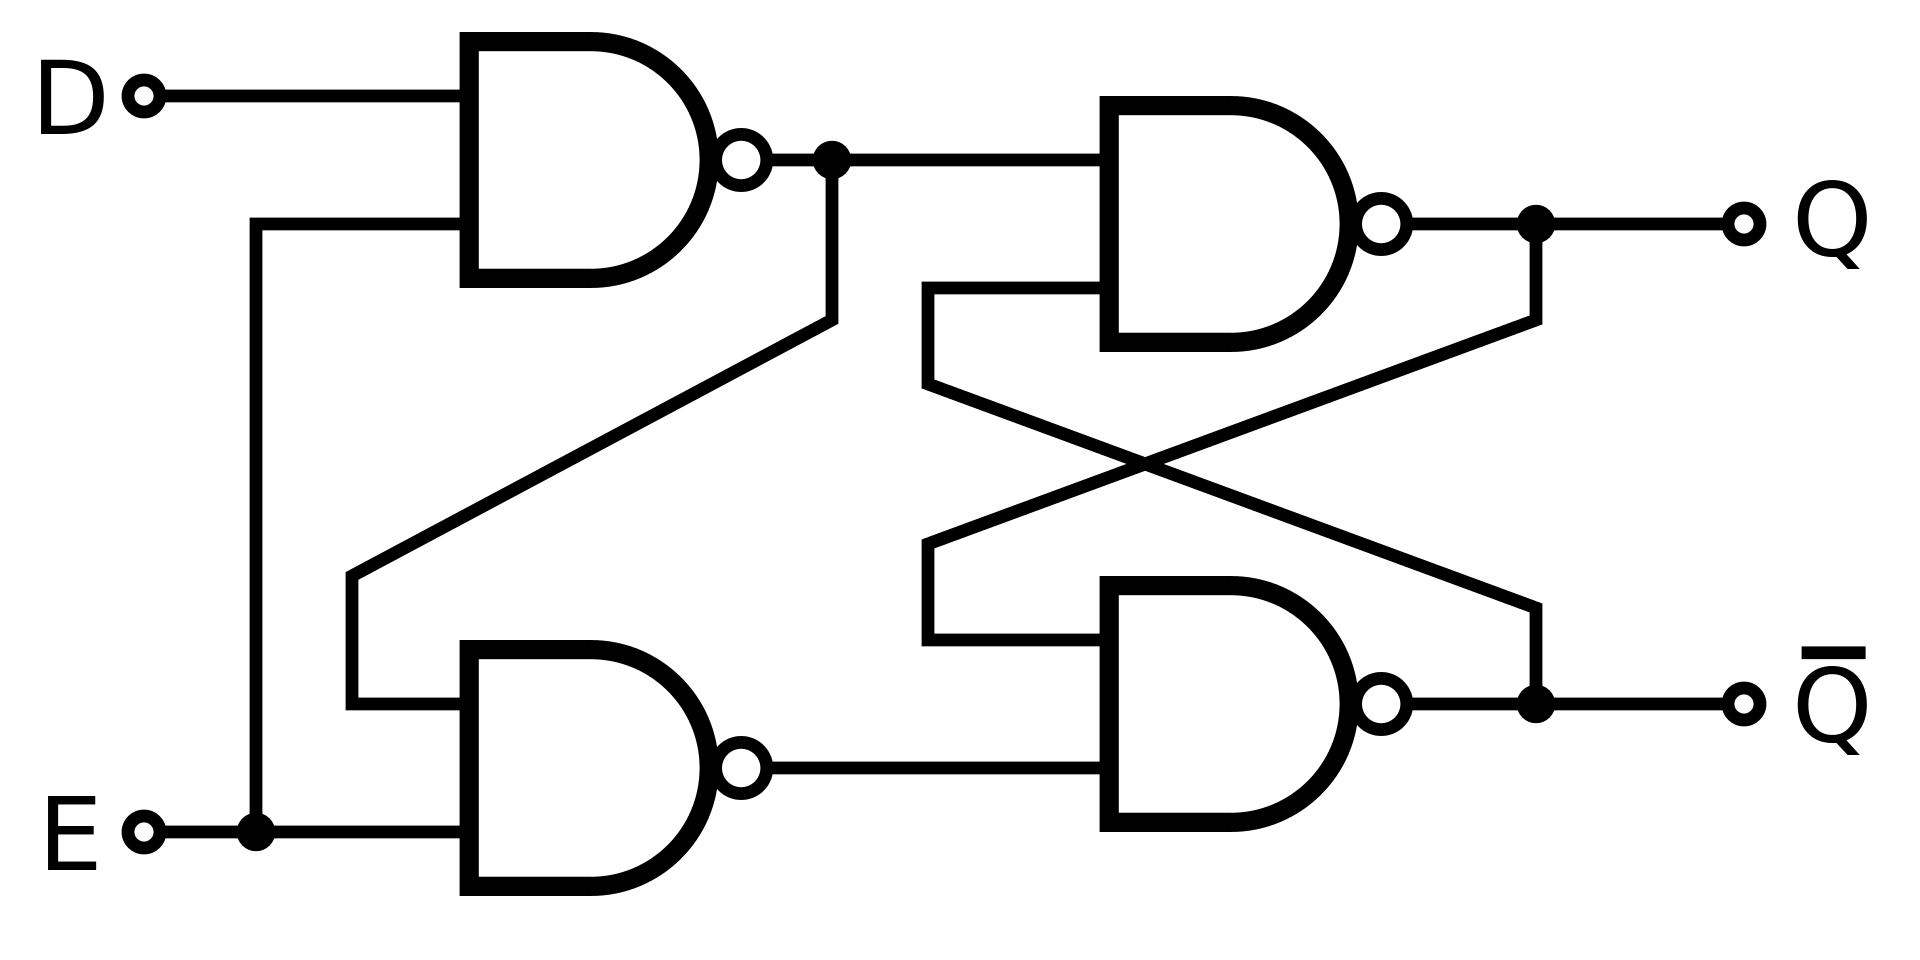
\includegraphics[width=.6\linewidth]{gated-d-latch.png}
		\begin{tabular}[!ht]{@{}cc|ccc@{}}
			\toprule
			$E/C$ & $D$ & $Q$               & $\overline{Q}$               & Comment   \\
			\midrule
			0     & X   & $Q_\textit{prev}$ & $\overline{Q}_\textit{prev}$ & No change \\
			1     & 0   & 0                 & 1                            & Reset     \\
			1     & 1   & 1                 & 0                            & Set       \\
			\bottomrule
		\end{tabular}
	\end{center}
	Operate on the principle of propagation delay.

	% REVIEW: Do we need this?
	% seems like a lot of space dedicated to something that's trivial to derive
	% from scratch
	Stacking many of them can be used to create a register:
	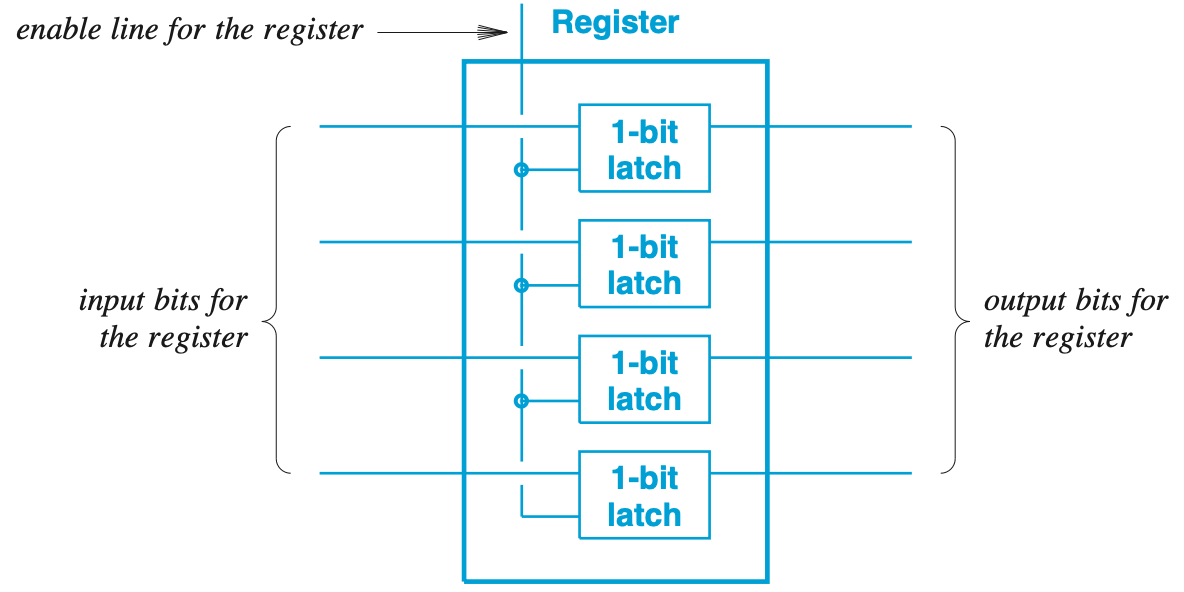
\includegraphics[width=\linewidth]{register.png}

	\subsection{Counters}
	For each transition from \textbf{low to high}, the counter increments the binary output by 1.
	(Counting the transition from high to low does the same thing, but the lecture used rising-edge counters).

	\subsection{Decoders}
	Take in an $n$-bit number, and turn on one of $2^n$ outputs.

	\subsection{Multiplexer / Demultiplexer}
	Turns $n$ signals into a single signal, and back on the other end.
	
	\subsection{Fixed \& Programmable Logic}
	\textbf{Fixed logic circuits:} Pre-determined function.
	\textbf{Programmable logic:} FPGAs (reprogrammable, but still a significant cost to switching functions).
	\textbf{Stored program and re-programmable circuits:} Your computer right now.
	\section{Data Encoding}
\end{multicols*}

\end{document}